\section{Results}\label{sec:results}

\subsection{Implied volatility does the work}

Table~\ref{tab:ladder} compares each model with HAR. Adding the VIX and MOVE
lowers the pooled mean squared error by 3.1\% at one day and 5.5\% at one
week, both highly significant, and by 1.8\% at one month, which is not. The
gains are broad: HAR-X beats HAR for 111 of the 115 stocks at the weekly
horizon.

\begin{table}[H]
\caption{Out-of-sample accuracy relative to HAR.}
\label{tab:ladder}
\footnotesize
\begin{tabularx}{\textwidth}{Xrrrrrr}
\toprule
& \multicolumn{2}{c}{$h=1$} & \multicolumn{2}{c}{$h=5$} & \multicolumn{2}{c}{$h=22$} \\
\cmidrule(lr){2-3}\cmidrule(lr){4-5}\cmidrule(lr){6-7}
Model & $\Delta$MSE & DM & $\Delta$MSE & DM & $\Delta$MSE & DM \\
\midrule
HAR & 0.6146 &  & 0.3381 &  & 0.2632 &  \\
HAR-X & +3.11\% & +5.23$^{***}$ & +5.54\% & +5.35$^{***}$ & +1.77\% & +0.95 \\
HAR + own persistence & -0.61\% & -3.77$^{***}$ & -0.09\% & -0.24 & -1.88\% & -3.21$^{***}$ \\
HAR + cross-sectional state & -0.23\% & -0.95 & +0.00\% & +0.01 & -1.61\% & -0.68 \\
HAR + sector state & -0.09\% & -1.71$^{*}$ & +0.13\% & +0.70 & -0.01\% & -0.03 \\
HAR + $d$, VIX, MOVE, $d\times$VIX, $d\times$MOVE & +2.89\% & +4.02$^{***}$ & +5.58\% & +4.47$^{***}$ & +0.41\% & +0.21 \\
Full model $C$ & +2.14\% & +2.58$^{***}$ & +5.79\% & +4.22$^{***}$ & -1.54\% & -0.64 \\
\bottomrule
\end{tabularx}
\noindent{\footnotesize{\textit{Notes:} Pooled out-of-sample MSE of log mean future Parkinson variance, 646 weekly origins (17 June 2013 to 14 April 2026) $\times$ 115 stocks, common cells. The HAR row reports its MSE; other rows the percentage reduction relative to HAR (positive is better) and the panel Harvey--Leybourne--Newbold Diebold--Mariano statistic. $^{*}$, $^{**}$, $^{***}$: 10\%, 5\%, 1\%.}}
\end{table}


The persistence blocks added to HAR, without implied volatility, do nothing
useful. Own-stock persistence worsens forecasts at the daily and monthly
horizons; the cross-sectional and sector states are indistinguishable from
zero. The specifications that do improve on HAR, $A_5$ and $C$, are those
that contain the VIX and MOVE, and their gains match HAR-X's. Model $C$'s
5.8\% at one week is HAR-X's 5.5\% plus a small amount, and at one month
model $C$ is worse than HAR. The breadth figures tell the same story: model
$C$ beats HAR for 107 stocks at the weekly horizon but for only 48 at the
monthly horizon.

\subsection{Persistence beyond HAR-X}

Table~\ref{tab:harx} tests the persistence terms directly against HAR-X. The
three registered extensions change the mean squared error by between
$-2.0\%$ and $+0.003\%$; none has a significant Diebold--Mariano statistic
in its favour, and at one month one is worse at the 5\% level and
another at the 10\% level. Model $C$ gains
0.26\% at one week ($t=0.41$) and is significantly worse at one day ($-1.0\%$,
$t=-2.14$) and one month ($-3.4\%$, $t=-2.69$).

\begin{table}[H]
\caption{Does persistence add to HAR-X?}
\label{tab:harx}
\footnotesize
\begin{tabularx}{\textwidth}{Xcrrrrr}
\toprule
Specification & $h$ & $\Delta$MSE & DM & CW & CW $p$ (Holm) & GW $p$ \\
\midrule
HAR-X + cross-sectional state$^{\dagger}$ & 1 & -0.03\% & -0.10 & +3.76$^{***}$ & 0.001 & 0.743 \\
 & 5 & +0.00\% & +0.01 & +4.44$^{***}$ & 0.000 & 0.923 \\
 & 22 & -2.01\% & -1.77$^{*}$ & +1.11 & 0.403 & 0.133 \\
\midrule
HAR-X + sector state$^{\dagger}$ & 1 & -0.10\% & -0.35 & +2.77$^{***}$ & 0.017 & 0.668 \\
 & 5 & -0.13\% & -0.34 & +2.49$^{***}$ & 0.032 & 0.543 \\
 & 22 & -0.86\% & -1.30 & +0.94 & 0.403 & 0.418 \\
\midrule
HAR-X + state $\times$ HAR terms$^{\dagger}$ & 1 & -0.37\% & -0.93 & +3.09$^{***}$ & 0.007 & 0.401 \\
 & 5 & -0.39\% & -0.66 & +2.44$^{***}$ & 0.032 & 0.282 \\
 & 22 & -1.77\% & -2.04$^{**}$ & +0.61 & 0.403 & 0.108 \\
\midrule
Full model $C$ & 1 & -1.00\% & -2.14$^{**}$ & +5.96$^{***}$ & 0.000 & 0.064 \\
 & 5 & +0.26\% & +0.41 & +8.31$^{***}$ & 0.000 & 0.697 \\
 & 22 & -3.37\% & -2.69$^{***}$ & +6.63$^{***}$ & 0.000 & 0.018 \\
\bottomrule
\end{tabularx}
\noindent{\footnotesize{\textit{Notes:} $\Delta$MSE: percentage reduction in pooled MSE relative to HAR-X (positive favours the specification). DM: panel HLN Diebold--Mariano statistic (two-sided). CW: Clark--West statistic for the nested comparison (one-sided). Holm adjusts the nine tests of the three pre-registered specifications ($^{\dagger}$) jointly and model $C$'s three tests jointly. GW: Giacomini--White conditional predictive ability test with instruments $(1, d_{t-k})$, $k=\lceil h/5\rceil$. All statistics use the cross-sectional mean loss differential per date and a Newey--West bandwidth of $\max(\lceil h/5\rceil-1,\lfloor 4(T/100)^{2/9}\rfloor)=6$.}}
\end{table}


The Clark--West statistics tell a different story at first sight. They are
large and positive for every specification at one day and one week, and the
Holm-adjusted $p$-values are below 0.05 for all three registered extensions
at those horizons. Formally, two specifications therefore meet the
registered rule: the cross-sectional extension at one week, with a gain of
0.003\%, and model $C$ at one week, with 0.26\%. Neither gain is
economically meaningful and neither meets the 0.5\% threshold we added after
seeing the results.

The two tests answer different questions, and the Giacomini--White test
resolves the apparent conflict. Clark--West asks whether the persistence
coefficients are zero in population; its adjustment removes the noise that
estimating them adds to the larger model's forecasts. A rejection says the
persistence terms are correlated with future variance once HAR-X is
controlled for. Giacomini--White asks whether the estimated model forecasts
better, conditionally on recent relative performance. It never favours a
persistence specification: the $p$-values for the registered extensions lie
between 0.11 and 0.92, and the only rejections, for model $C$ at one month
($p=0.018$) and nearly at one day ($p=0.064$), go against it. The information
the persistence terms carry is real but small, and estimating 11 extra
coefficients per stock costs more than it returns. Given
Section~\ref{sec:window}, this is the expected outcome: the state is largely
a smoothed function of past VIX extremes, which the VIX itself partly
reflects.

Figure~\ref{fig:cumulative} shows where the gains and losses accrue. The
value of implied volatility over HAR builds steadily at the daily and weekly
horizons, with jumps in March 2020. The value of persistence beyond HAR-X
drifts down at the daily and monthly horizons and stays near zero at the
weekly horizon, where its small positive balance arrives only in 2025.

\begin{figure}[H]
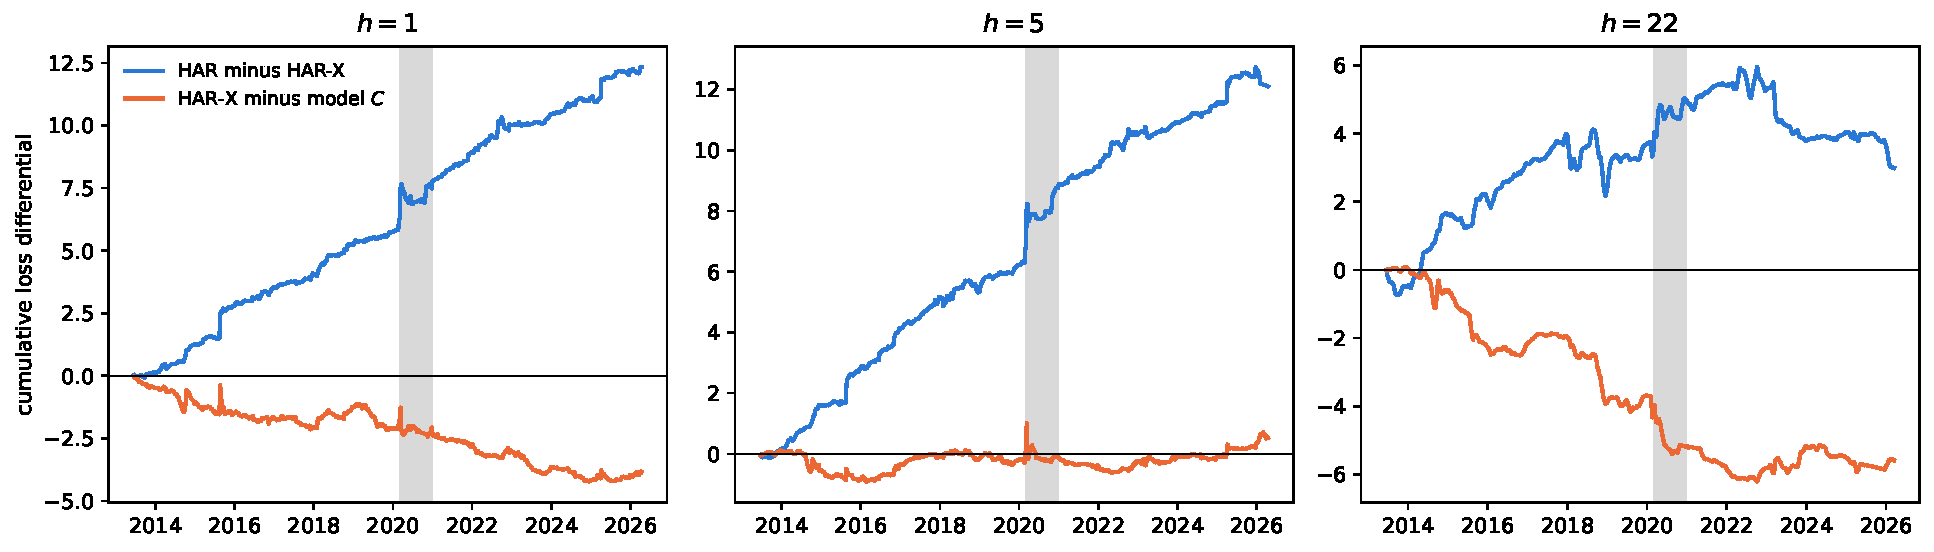
\includegraphics[width=\textwidth]{figures/fig_cumulative.pdf}
\caption{Cumulative sum over forecast origins of the cross-sectional mean
squared-error differential. Blue: HAR minus HAR-X (rising when implied
volatility helps). Orange: HAR-X minus model $C$ (rising when persistence
helps beyond implied volatility). Common cells; shading marks March to
December 2020.}
\label{fig:cumulative}
\end{figure}

\subsection{Information timing}

The comparison between HAR and HAR-X is sensitive to a detail that is easy
to get wrong. If the HAR terms are built from variance through day $t-1$,
for example by lagging the regressors one day to avoid look-ahead, while the
VIX is the close of day $t$, the implied-volatility model receives one more
day of information than the benchmark. Table~\ref{tab:timing} re-estimates
both models with HAR inputs ending at $t-1$ and compares them with the
aligned versions used elsewhere in the paper.

\begin{table}[H]
\caption{Information timing and the apparent value of implied volatility.}
\label{tab:timing}
\small
\begin{tabularx}{\textwidth}{Xcrrr}
\toprule
HAR inputs & $h$ & MSE HAR & MSE HAR-X & HAR-X gain (DM) \\
\midrule
Through $t-1$ & 1 & 0.6691 & 0.6350 & +5.11\% (+4.56) \\
 & 5 & 0.3637 & 0.3354 & +7.76\% (+4.62) \\
 & 22 & 0.2712 & 0.2633 & +2.90\% (+1.46) \\
\midrule
Through $t$ & 1 & 0.6146 & 0.5955 & +3.11\% (+5.23) \\
 & 5 & 0.3381 & 0.3193 & +5.54\% (+5.35) \\
 & 22 & 0.2632 & 0.2586 & +1.77\% (+0.95) \\
\midrule
HAR, $t$ vs $t-1$ & 1 & & & +8.15\% (+6.39) \\
 & 5 & & & +7.04\% (+5.00) \\
 & 22 & & & +2.93\% (+3.41) \\
\bottomrule
\end{tabularx}
\noindent{\footnotesize{\textit{Notes:} VIX and MOVE are closes of the origin day $t$ in every row. Through $t-1$: HAR terms built from variance through the day before the origin and the previous day's return. Through $t$: the aligned specification used everywhere else. Common cells of all four forecast panels; DM statistics in parentheses.}}
\end{table}


Aligning the inputs lowers HAR's error by 8.1\% at one day, 7.0\% at one week
and 2.9\% at one month, all significant. Because HAR-X already contains the
day-$t$ VIX, it gains less from the alignment, and its advantage over HAR
falls from 5.1\% to 3.1\%, from 7.8\% to 5.5\% and from 2.9\% to 1.8\%. Between
29\% and 39\% of the apparent value of implied volatility is a timing
artefact. Earlier versions of this study used the misaligned convention and
reported the larger gains; any study that compares HAR with implied-volatility
regressors should check the same alignment.

\subsection{Three designs that give persistence a better chance}

Three objections to the per-stock design are natural, and Table~\ref{tab:designs}
answers each with a design registered before its results were computed.

\begin{table}[H]
\caption{Three designs that give persistence a better chance.}
\label{tab:designs}
\footnotesize
\begin{tabularx}{\textwidth}{lXcrrr}
\toprule
Design & Comparison & $h$ & $\Delta$MSE & DM & CW $p$ (Holm) \\
\midrule
Pooled, fixed effects & Full model vs HAR-X & 1 & +0.40\% & +1.19 & 0.000 \\
 &  & 5 & +0.34\% & +0.79 & 0.000 \\
 &  & 22 & -1.36\% & -1.30 & 0.627 \\
 & HAR-X + cross-sectional state vs HAR-X & 1 & +0.34\% & +1.18 & 0.004 \\
 &  & 5 & +0.19\% & +0.53 & 0.016 \\
 &  & 22 & -1.00\% & -0.96 & 0.627 \\
\midrule
Duration target & Full model vs HAR-X & 22 & -1.81\% & -3.92$^{***}$ & 0.026 \\
 & HAR-X + cross-sectional state vs HAR-X & 22 & -0.35\% & -1.42 & 0.677 \\
\midrule
Market level & Full market model vs market HAR-X & 1 & +3.42\% & +1.77$^{*}$ & 0.000 \\
 &  & 5 & +2.01\% & +1.45 & 0.000 \\
 &  & 22 & -1.93\% & -1.00 & 0.270 \\
\bottomrule
\end{tabularx}
\noindent{\footnotesize{\textit{Notes:} Pooled: one regression across stocks with stock fixed effects (within transformation on training means), refit at every origin. Duration target: log ratio of mean future variance over 22 and 5 days. Market level: one series, the cross-sectional mean of the stock targets, with market HAR terms, VIX, MOVE and the persistence state. Each design was specified before its results were seen.}}
\end{table}


First, per-stock regressions estimate many coefficients from about 650 weekly
observations, and the persistence state is common to all stocks. A pooled
regression with stock fixed effects estimates each coefficient once from the
whole panel. Pooling helps: model $C$ now beats pooled HAR-X by 0.40\% at one
day and 0.34\% at one week, and the Clark--West rejections survive Holm
adjustment. But the gains are well below the 0.5\% threshold and not
significant by Diebold--Mariano, and at one month the sign reverses.

Second, persistence might describe how long volatility stays high rather
than how high it is. We therefore forecast the slope of the variance term
structure, the log ratio of mean variance over the next 22 days to mean
variance over the next 5. HAR beats an expanding-mean benchmark on this target
by 3.3\%, so the slope is forecastable, but adding persistence to HAR-X makes the
forecasts worse, significantly so for model $C$ ($-1.8\%$, $t=-3.92$).

Third, the state is a market-wide quantity and may be visible only at the
market level. On a single series, the cross-sectional mean of the stock
targets, the persistence state improves on a market HAR-X by 3.4\% at one day
and 2.0\% at one week, with Diebold--Mariano statistics of 1.77 and 1.45. This
is the largest gain in the study, but with one series and 646 origins it is
not significant, and Appendix~\ref{app:market} shows that it is carried by a
known quantity: the trailing gap between implied and realized variance,
which captures the variance risk premium, absorbs it.

\subsection{Calm and stressed periods}

Splitting the evaluation period by the quartiles of the VIX on the forecast
dates gives no sign of a regime in which persistence pays. In the highest
VIX quartile model $C$ improves on HAR-X by 2.4 percentage points at one week,
with a Diebold--Mariano statistic of 1.36; in the lowest quartile it is
worse at every horizon; during March to December 2020 it is 0.2 points
worse at one week and 5.6 points worse at one month. With 162 dates per
quartile and 43 in 2020 these comparisons are descriptive.
